\documentclass[a4paper]{report}
\usepackage{graphicx}
\graphicspath{{J:/report/appendixImages/}}
\begin{document}


\title{Goal Orientated Action Planning Artificial Intelligence}
\author{Sam McKay \and Illiyan Georgiev \and ‎José Diez\and Vlad-Eugen Tanase \and Aaron Swiss-Hamlet }
\maketitle
\tableofcontents
\chapter{Introduction}
Project 10 of the 206CDE Real World Projects, namely Goal Orientated Action Planning (GOAP) for Game Artificial Intelligence (AI) was successfully finished by this group. In this project, we will discuss the GOAP artificial intelligence type and its uses within video games. This project was complete in eight months by a team consisting of five members. Due to the majority of the team belonging to the Games Technology course, the overall look and feel of the project is similar to a two-dimensional pixel art style video-game, although no player interaction is possible. 
 
GOAP AI refers to a simplified STRIPS-like planning architecture, designed for real-time control of various character behaviours within video games. A good example of a GOAP AI is the F.E.A.R. video-game AI, which has won many awards and is acclaimed as one of the best gaming AIs. Various programs were used in the making of this project. The coding behind everything was done using the C++ programming language. Photoshop was used to develop various textures and sprites to be used in the game-like presentation. For graphical purposes, the Simple and Fast Multimedia Library (SFML) was used, which is based on the Open Graphics Library. Axosoft and GitHub were used for team organisation and progress tracking.

\chapter{Project Brief}
\chapter{Aims and Objectives}
The aim of this project is to create a goal orientated action planning artificial intelligence(AI) agent. This agent should be able to asses its current state against its goal state. Our AI agent should then begin to generate an action plan, that it will execute in order to achieve the desired state. \newline

\begin{itemize}
	\item Design and Create a Survival Game
	\item Create an Artificial Intelligence Agent capable of making an action plan
	\item Have the Artificial Intelligence Agent carry out the plan 
\end{itemize}

To demonstrate this we set ourselves the objective of designing and creating a survival game in which the main character is our AI agent. This world should be a desolate environment with multiple biomes and various resources all scattered about it, all of which is randomly generated to ensure our AI agent has a new challenge every time. With this world we envisioned in mind our next objective was to create a list of relevant actions for our AI to carry out. These actions should have pre and post conditions such that our AI could create multi action plans in order to complete a task such as satisfying its need for hunger. To be able to generate these plans we would need to create a planer algorithm, for this we would use similar logic to the STRIPS implementation around which the majority of our research was based. Finally our last objective is that we need to be our able to visualize our AI agent planning and carrying out these plans. To show this we would use the SFML library to graphically represent the aforementioned environment, along with a user interface to show the AI agents "thought process".
 
\chapter{Project Management}
In order for this project to succeed we needed to implement an effective project management methodology. For this we chose to implement the agile project management structure commonly used within the software industry. Due to the size and length of the project it was imperative that we implemented good project management from the beginning, without it we could have struggled to complete the project in a timely, well paced fashion. By ensuring we had this project management in place from the start it meant that we could track our progress and continue to work at a reasonable pace throughout the duration of the project.

Agile project management is a highly effective method of managing long term projects, the process can be broken down into many stages. To begin with you collect all of your user stories, or feature requests, into a product backlog. These user stories are mostly generated by members of the team and define the "wish list" of features to include in the project. Once we have all our user stories we can begin selecting the features we will include in the final product into a release backlog (see Appendix 1.01). This release backlog can be broken down into various stages known as sprints, these sprints can be as long as a couple of days up to a whole month. All of these sprints come together to create the full product with each sprint generally expanding upon the work completed in the previous sprint.

In order for teams to easily implement this project management methodology, various different companies have all produced their own software to provide the agile management approach. We chose to use \textit{Axosoft's} Scrum software, this creates a personalised website for the team to use and grants access to all of the previously discussed features. Using this we quickly created all of our user stories and proceeded to arrange these into various different sprints. We decided upon five sprints for the project: Research, Planning, Design and two programming sprints. This helped us to ensure that we kept on track as each task as an estimate for how long it will take to complete. So as work is done on each task we attach a work log to it and can compare estimated time with the actual duration of the task and use that as a measure of when we will finish the project as a whole using a burn-down chart (see Appendix 1.02)

By using Scrum we were able to monitor our progress and even predict release dates, which helped to give us something to aim for. We were also able to track who was working on what and exactly what work has been done on each section as well as what is left to be done. This meant that we didn't have two people each working on exactly the same task and prevented wasting time by doing so. Without Scrum it would have been very challenging to know exactly what stage we were all at and what needed to be done to meet the next deadline. Scrum also helped with our testing process by providing a bug tracker (see Appendix 1.03), allowing us to easily track any bugs and to test new code as it was completed. 

We also made use of GitHub, a code sharing repository, in order to store and share our code amongst the team. This allowed us to organise the code and maintain version control whilst also enabling the team to work on various sections at the same time. Throughout the project weekly meetings were attended, Monday with the project supervisor. Team meetings were established by the project manager based on necessity and the availability of every member, minimum once a week. On various occasions, more than one meeting was booked within the library to work, discuss or establish new tasks.

PLANNING?


\chapter{Methodology}
\subsection{Design Methodology}
The design methodology has meant implementing a process whereby the entire team has had some input into the creation of the program’s design, both structurally and graphically. In the initial research stage of the project, this meant looking up existing user interfaces (referred to as the UI from now) and determining what kind of art style the program would have to determine the best way to present the information to the screen. Interfaces that were looked at include the World of Warcraft system and how its pre-set setup was not favoured due to a lack of specific information and that of The Sims, where the needs of each sim are covered in the simple design of the UI. Fitting the graphical design to the needs of the project requirements, taking an approach much like The Sims seemed appropriate as this provides a simple and easy to understand system for users to see. The next aspect to approach on the design aspect is that of the world’s graphical look. This needed to compliment the UI design. Due to the amount of time available for the entire project as well as the size of our team, a 2D world approach made more sense, which formed the basis of our initial strategy for approaching the project.

Once past the research and initial concept stage, the design implementations need to be coupled with the programming side of the project in the planning and prototyping stage. This meant talking as a group, with each member of our team to come up with the best solution to the design challenges presented. These include showing elements of the AI’s thought processes to the screen. Furthermore, aspects of the AI itself that affect its planning and how to represent the items it has on its person to use. Approaching the thought processing aspect, there are many elements that the AI could need to do, for example, obtaining wood or needing to sleep. Therefore, as there are a large variety of different actions that the AI can perform, trying to graphically represent everything in a list is not a good method of display. Therefore the next best method would be to display its thoughts in a console statement window.

The next element to address in the planning stage is the way in which the AI will have elements that affect it displayed to the screen. This means visually representing to the user what exactly is making the AI decide to do that action. As this design aspect includes programming limitations, both sides of the project needed to come together on this segment. Too many elements, which we decided to call “weights”, would make programming the AI too hard for the timeframe we had. On the hand too little would not give the AI anything to work on or react to within the environment. Therefore, we decided upon using only the core aspects of a human as the weights which we would include in the program. As such, four of these are included in the final simulation: hunger, thirst, energy and warmth. These were whittled down from a larger list of weights which were the initial criteria we were going to go with however, this makes for a much simpler AI system that fits the expected project outcomes. In order to demonstrate these weights to the user, we chose to use a coloured background that changes under certain conditions. This was favoured over using a bar that changes in size as this is an obvious visual representation that is instantly clear to viewers.

The final element of the UI was to display what the AI has on its person, whether it be food or a material used in creating a fire or shelter. This was much like the appearance of the weights on the UI as they can be used with a simple tile that sticks out from the rest of the UI around it. As evidenced in the final design proposal, there are tiles intended for inventory space with the ability to remove them easily as needed due to not interacting with any other element in the program's environment.

The final graphical design challenge is the creation of the 2D environment that the AI will work within. This requires a simple implementation of images that act as “tiles” in the world to create a randomly generated world where there are a selection of biomes across a fixed space environment. To create these biomes, an xml map generator is created using a sub program that denotes which biome is where, and the image that represents the biome on that tile will be displayed based on the programming implementation. Once the map is implemented, the graphics are placed in the world and then the program generates the world. On top of the terrain tiles that are produced, there are .png files which denote resources in the world, such as trees and stone, that are placed on top of the terrain under conditions that the resource has to have fulfilled before it spawns in that tile. Keeping the amount of resources in the world was essentially due to the timeframe and also for the implementation of other aspects in the program on the technical side. These tiles are equal in size, being 64x64 pixels and take a uniform art style which, while simple and not professionally impressing, still presents the world in an obvious manner to viewers of the program.
\subsection{Development Philosophy}
\subsection{Code Structure}
\subsection{Navigation}
\subsection{Simple and Fast Multimedia Library}
\subsection{Map Generation}
For this project, a random map generator has been created. The size of the map in height and width is necessary, as well as the number of biomes to be created. Afterwards, each biome must have an individual, distinguishable character such as "\#" or "*" and a limit of spaces this biome can take. The generator sets the starting position of each biome, with a minimum distance between each biome. The map starts with a default empty biome, drawn with the blue colour. After each position is set accordingly, the drawing starts from the middle, using the limit to take the spaces and checking if the spaces are not used by any other biome except the default one.	At the end of the generation, the map is shown using the SFML for graphical representation and an eXtensible Markup Language file is generated, containing the number of biomes, height and width, as well as every tile data type.

The Resource generation program imports and reads the XML file in order to determine the map and biomes associated to it. Each resource has a limit as well, and can only be assigned to one biome type. Once these are set, a random number is chosen between 0 and 3. With this number, the generation of the map will start from a specific corner of the map, such as 0 being top left, 1 being top right. Each resource is constrained to be spawned on an empty space and not have any other resource in its adjacency. A random number is generated every time a suitable position is found, and if it is 1, the resource is placed. A different XML file, containing the resource information of the map is generated at the end. With this imported into the main project, we have a randomly generated map populated with resources for the AI to use.

This was done in order to test the AI in different scenarios, in random maps with randomised resources in order to get different results, actions and plans from the AI. Even though every generation is random, some control is still available through coding if a resource or biome type should fit a certain criteria is needed, as well as the ability to modify the XML file itself to change the positions or types of any biome tile or resource.

\chapter{Testing}
\chapter{Discussion}
Overall the workflow of this project went smoothly. A large portion of the work has been done in the early stages, resulting in a base for future endeavours. Due to a team member using the Linux Operating System, various steps were taken in order to make future merging of work much easier. As such, after the first attempt, all other programming merges were done without any problems. 

Through the use of \textit{Axosoft} the organisation of the team was made significantly easier. This was updated almost daily by the project manager, and each specific card was updated timely and finished accordingly. A burn-down chart(see appendix 1.01) was available, determining the time at which the project would be done according to our work submitted and number of hours left on the remaining tasks. Effective use of GitHub was in turn used to organise the project from a programming point of view. Commits to individual branches were made regularly (see appendix 4.01) with each new project part or feature implemented. This provided every member with the ability to download and work with the latest version of the project from anywhere, as well as synchronise with the other programmers.

SFML was chosen for graphical representations due to its ease of use and efficiency. It is based on the Open Graphics library and was easy to implement within the project and used to drawn the map, resources and the AI. Visual representation was not highly necessary, yet it is useful, and allowed us to develop other various skills such as creating assets and implementing them accordingly.

Various different actions can be completed, such as gathering resources such as wood and being able to use the available resources. The AI will create a plan and then proceed to execute it. The resources are displayed via the interface to the user in the Inventory section, on the bottom left corner of the screen. Due to the nature of the project, other actions can be programmed with ease within the AI, giving it a much wider array of possible plans. Various assets are available within the project yet not used by the AI, such as a fireplace that can be built using wood and used to either cook food or generate warmth in order to satisfy one of the weights, namely the Warmth weight.

\chapter{Conclusion}
The project was successful in implementing a GOAP AI capable of planning and organising actions in order to complete a goal. The AI can be tested on various maps with different conditions in order to get different results based on the resources available to the AI. 
\chapter{Bibliography}
\appendix
\chapter{Appendix}
\section{}
\subsection{}
	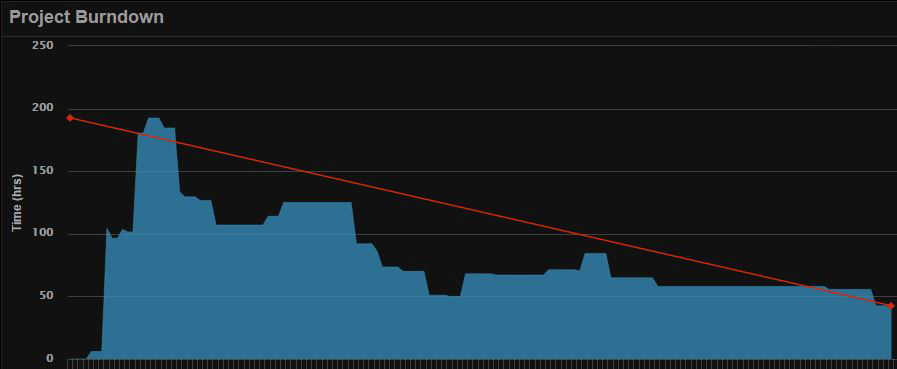
\includegraphics[width=1.0\linewidth]{./appendixImages/AxosoftScreenShot01}
	\textit{Axosoft} Burn-down Chart 
\subsection{}
	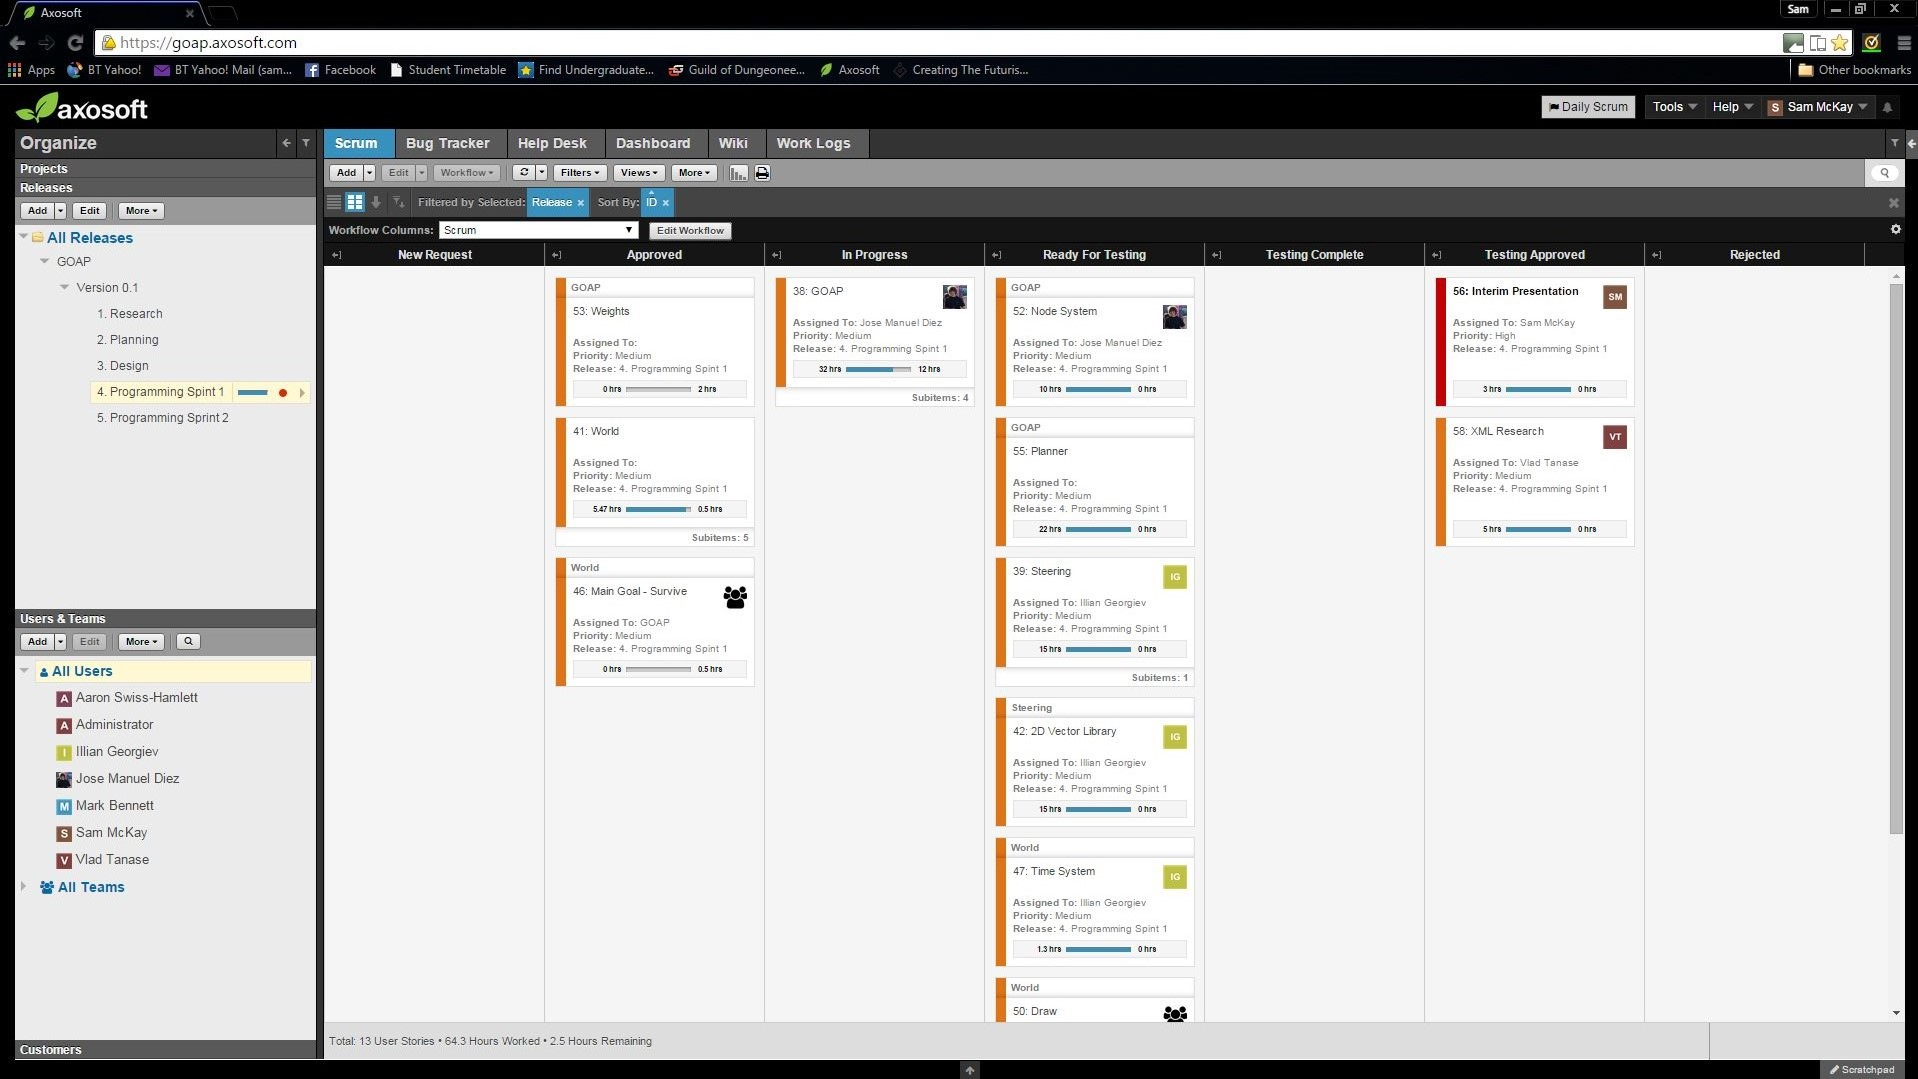
\includegraphics[width=1.0\linewidth]{./appendixImages/AxosoftScreenShot02}
	\textit{Axosoft} User Stories
\pagebreak
\section{}
\pagebreak
\section{}
\pagebreak
\section{}
\subsection{}
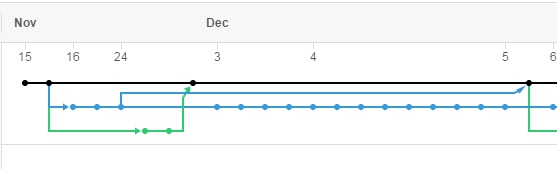
\includegraphics[width=1.0\linewidth]{./appendixImages/GitHubScreenShot01}
GitHub Branches
\pagebreak
\section{}

\end{document}